\documentclass[a4paper]{article}
\usepackage{geometry}
\geometry{left=2.0cm, right=2.0cm, top=1.5cm, bottom=1.5cm}
\usepackage[utf8]{inputenc}

\usepackage{hyperref}

\usepackage{amsmath}
\usepackage{amsfonts}
\usepackage{amssymb}
\usepackage{amsthm}
\usepackage{bbm}
\usepackage{interval}
\intervalconfig{
soft open fences
}
\usepackage{mathabx}
\theoremstyle{definition}
\newtheorem{definition}{Definition}[section]
\newtheorem{example}{Example}[section]
\newtheorem{lemma}{Lemma}[section]
\newtheorem{theorem}{Theorem}[section]
\newtheorem{corollary}{Corollary}[section]
\newtheorem{remark}{Remark}[section]

\usepackage{graphicx}
\usepackage{float}
\usepackage{caption}

\setlength\parindent{0pt}

\title{Deep RL Assignment1}
\author{Mufei Li \href{mufei.li@nyu.edu}{mufei.li@nyu.edu}}
\begin{document}
\maketitle

\section{Warmup}

We use the default setting in run$\rule{0.15cm}{0.15mm}$expert.py for collecting data. The setting for behavioral cloning is 
\begin{itemize}
\item \textbf{random seed}: $0$
\item \textbf{batch size}: $64$
\item \textbf{learning rate}: $0.001$
\item \textbf{number of epochs}: $10$
\item \textbf{shuffle}: The dataset is reshuffled at every epoch.
\item \textbf{optimizer}: Adam with its default setting in PyTorch $0.4.0$
\item \textbf{model}: a fully connected neural network with one hidden layer followed by a leaky ReLU using its default setting in PyTorch. Let an observation of the environment being $d$-dimensional. The number of parameters for the hidden layer is set to be $20d$.
\end{itemize}

The learning curve of the training plotted in TensorBoard is presented below:

\begin{figure}[H]
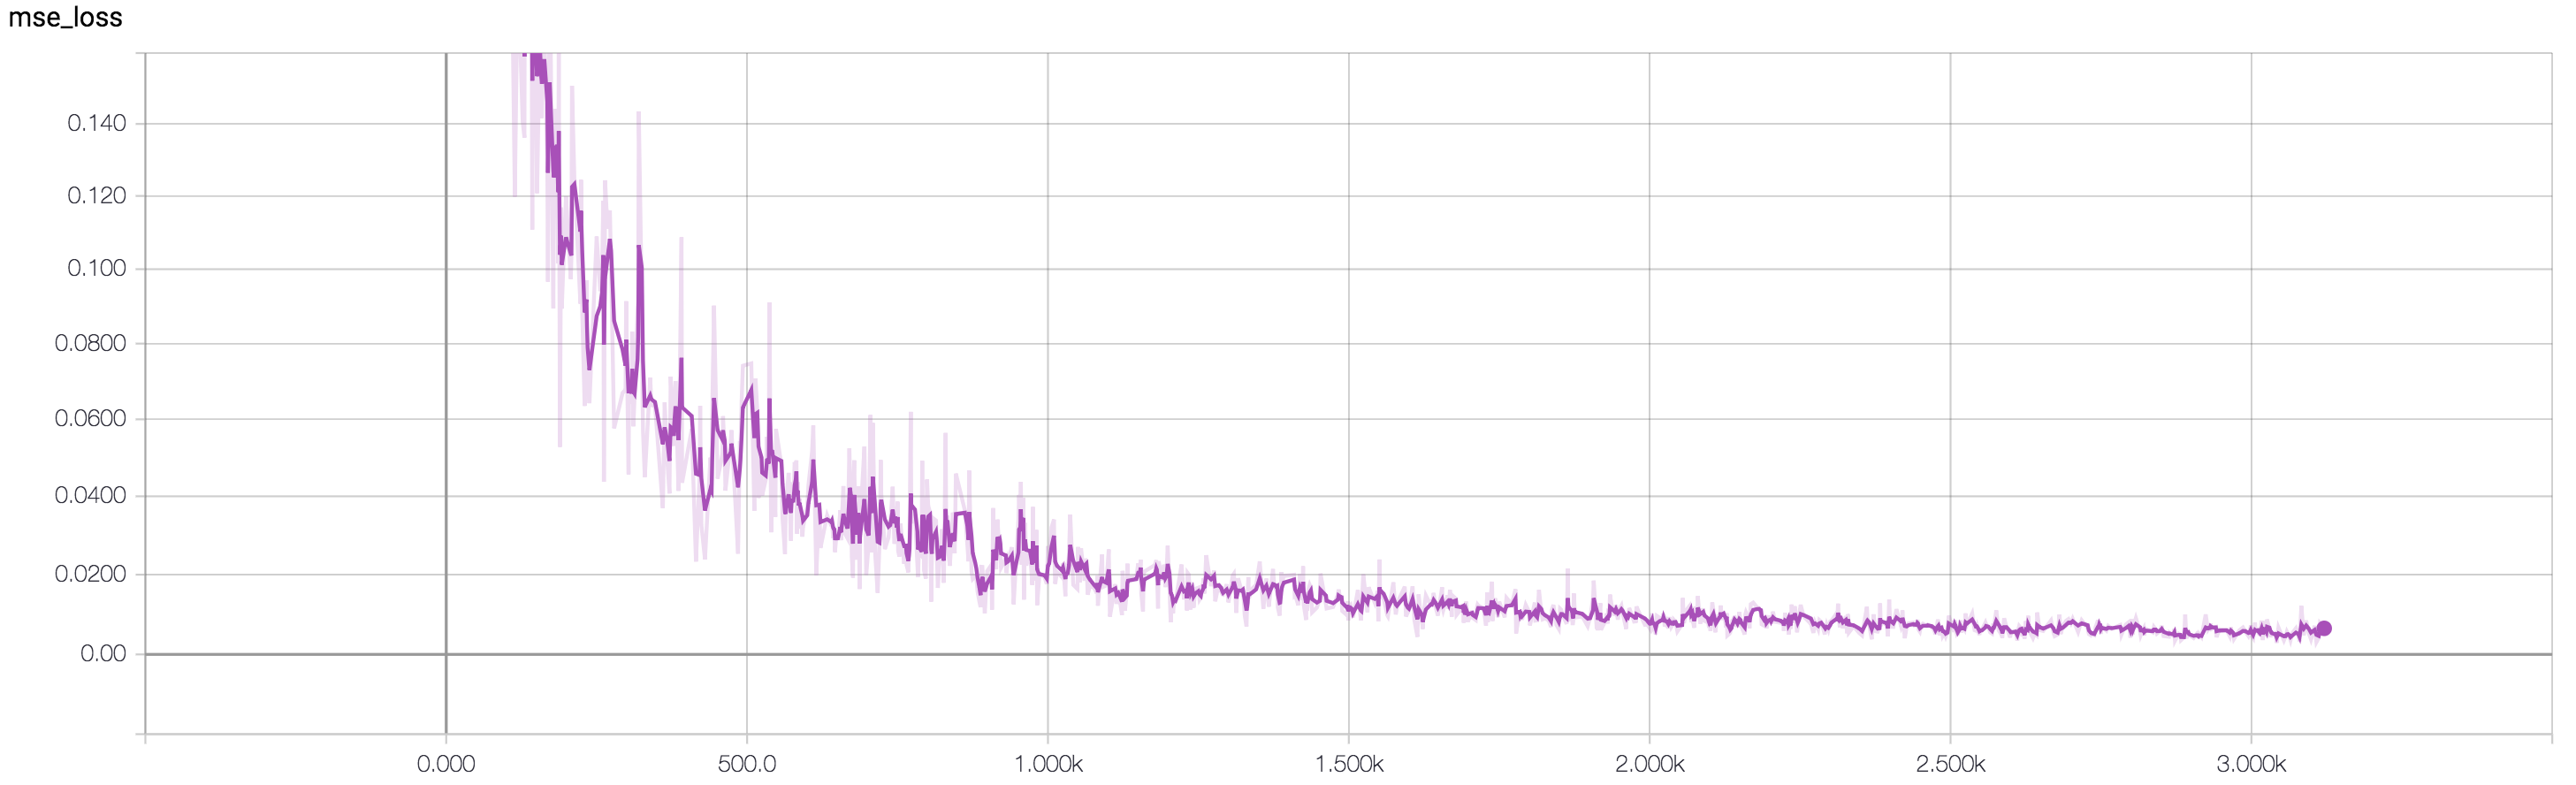
\includegraphics[width=\textwidth]{warm_up.png}
\caption{The learning curve for warmup.}
\end{figure}

\section{Behavioral Cloning}

\subsection{}

\begin{figure}[H]
\centering
\begin{minipage}{.5\textwidth}
  \centering
  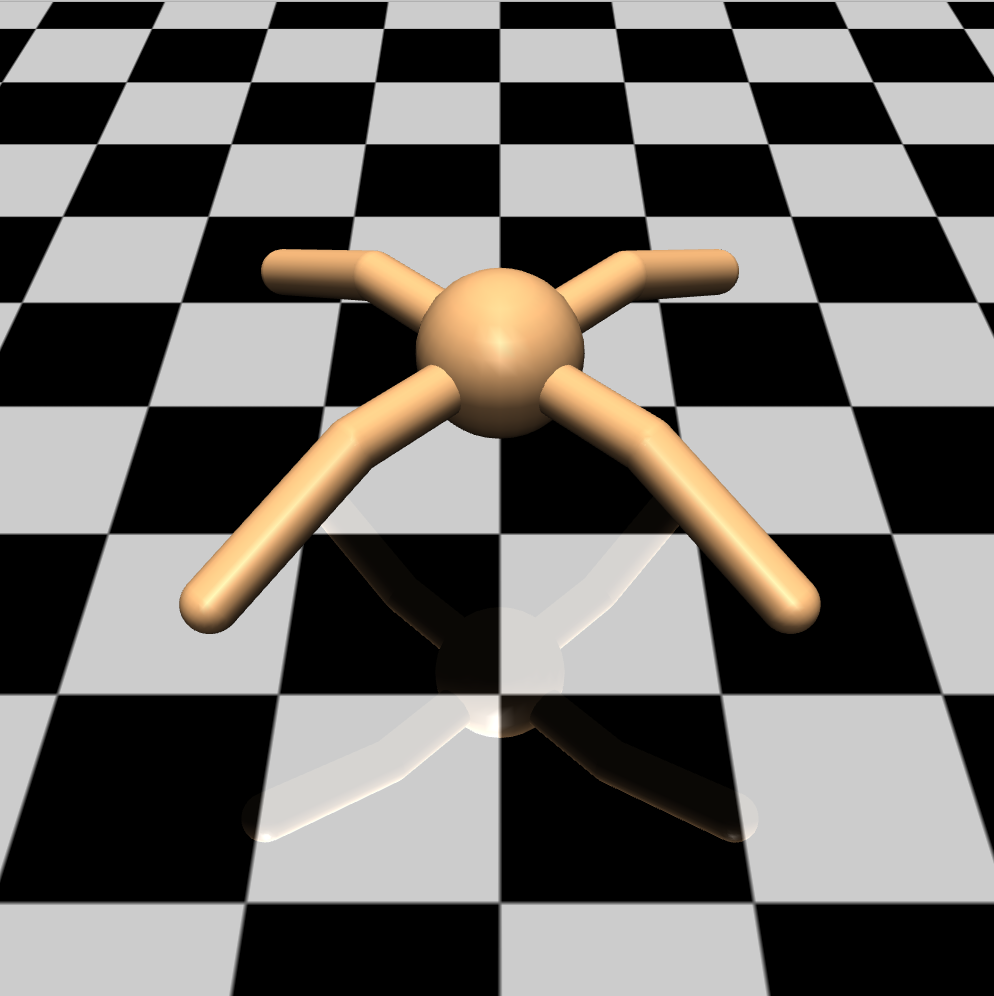
\includegraphics[width=0.4\linewidth]{Ant-v1.png}
  \captionof{figure}{Ant-v1}
\end{minipage}%
\hfill
\begin{minipage}{.5\textwidth}
  \centering
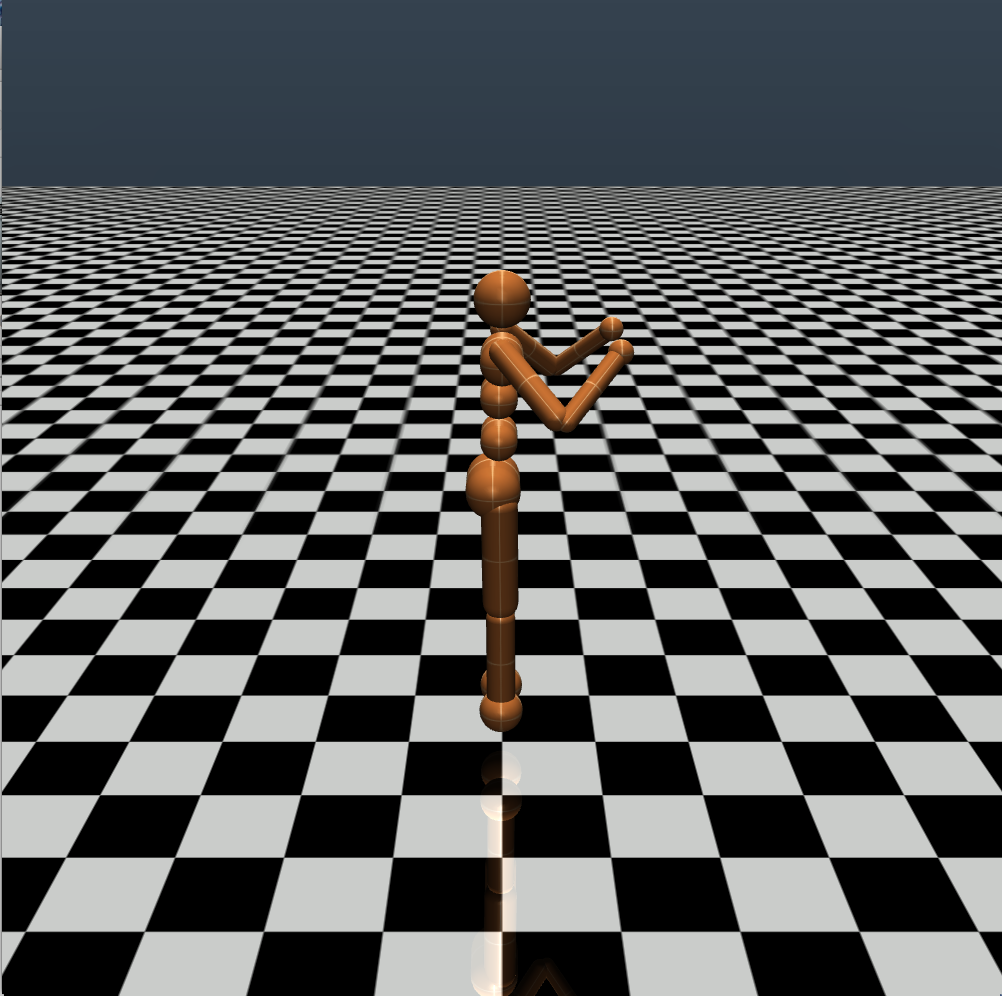
\includegraphics[width=0.4\linewidth]{Humanoid-v1.png}
\captionof{figure}{Humanoid-v1}
\end{minipage}
\end{figure}

The tasks we used for this question are \textbf{Ant-v1} and \textbf{Humanoid-v1}. The setting for the experiments is the same as in the warmup section. The statistics for both the expert and the trained (cloned) policy in the table\footnote{The numbers for the observation space and the action space simply indicate the dimension of the spaces.} below are calculated based on $20$ rollouts.\\

\begin{center}
\begin{tabular}{ |p{2.1cm}||p{1.8cm}|p{1.8cm}|p{1.8cm}|p{1.8cm}|p{1.8cm}|p{1.8cm}| }
 \hline
 Tasks& Observation Space& Action Space& Expert Mean& Expert Std& Cloned Mean& Cloned Std\\
 \hline
 Ant-v1 &111 &8 &4836.24 &123.77 &4639.13 &536.92\\
 Humanoid-v1 &376 &17 &10417.81 &57.65   &278.59 &65.72\\
 \hline
\end{tabular}\\
\end{center}

\bigskip
The performance we obtained in Ant-v1 is comparable to that of the expert policy, but it is clearly not the case for Humanoid-v1. 

\subsection{}

We experiment with different \textbf{random seeds}. Random seed, being one of the most influential hyperparameters, affects both the weight initialization for PyTorch as well as environment initialization in OpenAI's Gym. To my knowledge, deep reinforcement learning (DRL) approaches, particularly policy gradient methods, are very sensitive to random seeds. On the contrary, imitation learning is intuitively more of the style of supervised learning despite that the tasks in hand may be the same. It is therefore interesting to explore how random seeds affect the performance of behavioral cloning.\\

As the performance of behavioral cloning on Humanoid-v1 is significantly worse than that of the expert policy in the previous part, we choose this task for our experiment. During the experiment, we fix a collection of demonstrations from the expert policy and use exactly the same setting of the experiment as before except that we try $10$ random seeds: $0, 1,\cdots,9$. For each choice of random seed, we set the seed for both PyTorch and Gym environment. The results of the experiment are presented below:

\begin{figure}[H]
\centering
\begin{minipage}{.5\textwidth}
  \centering
  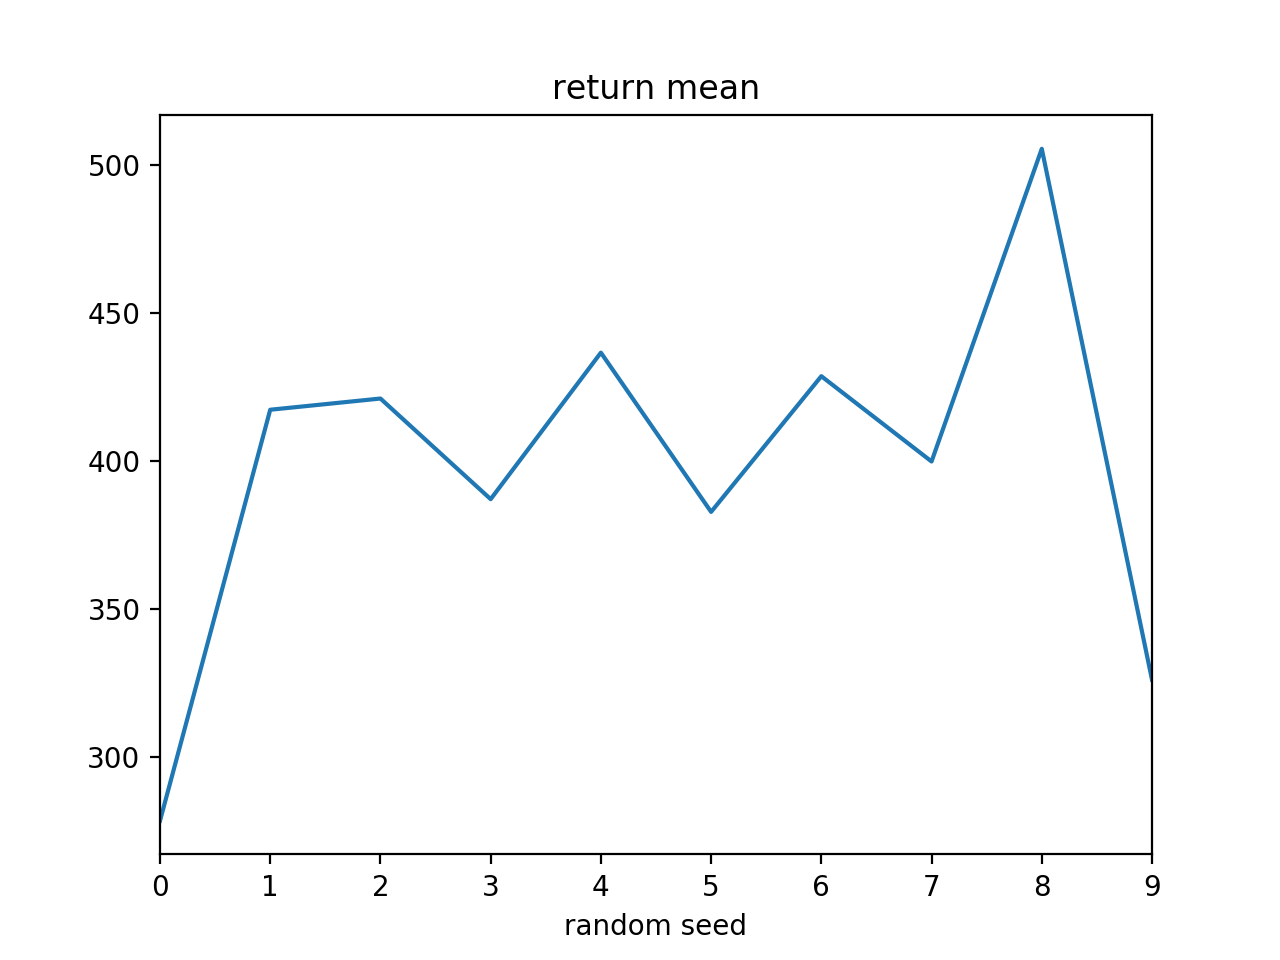
\includegraphics[width=0.95\linewidth]{return_mean.png}
  \captionof{figure}{}
\end{minipage}%
\hfill
\begin{minipage}{.5\textwidth}
  \centering
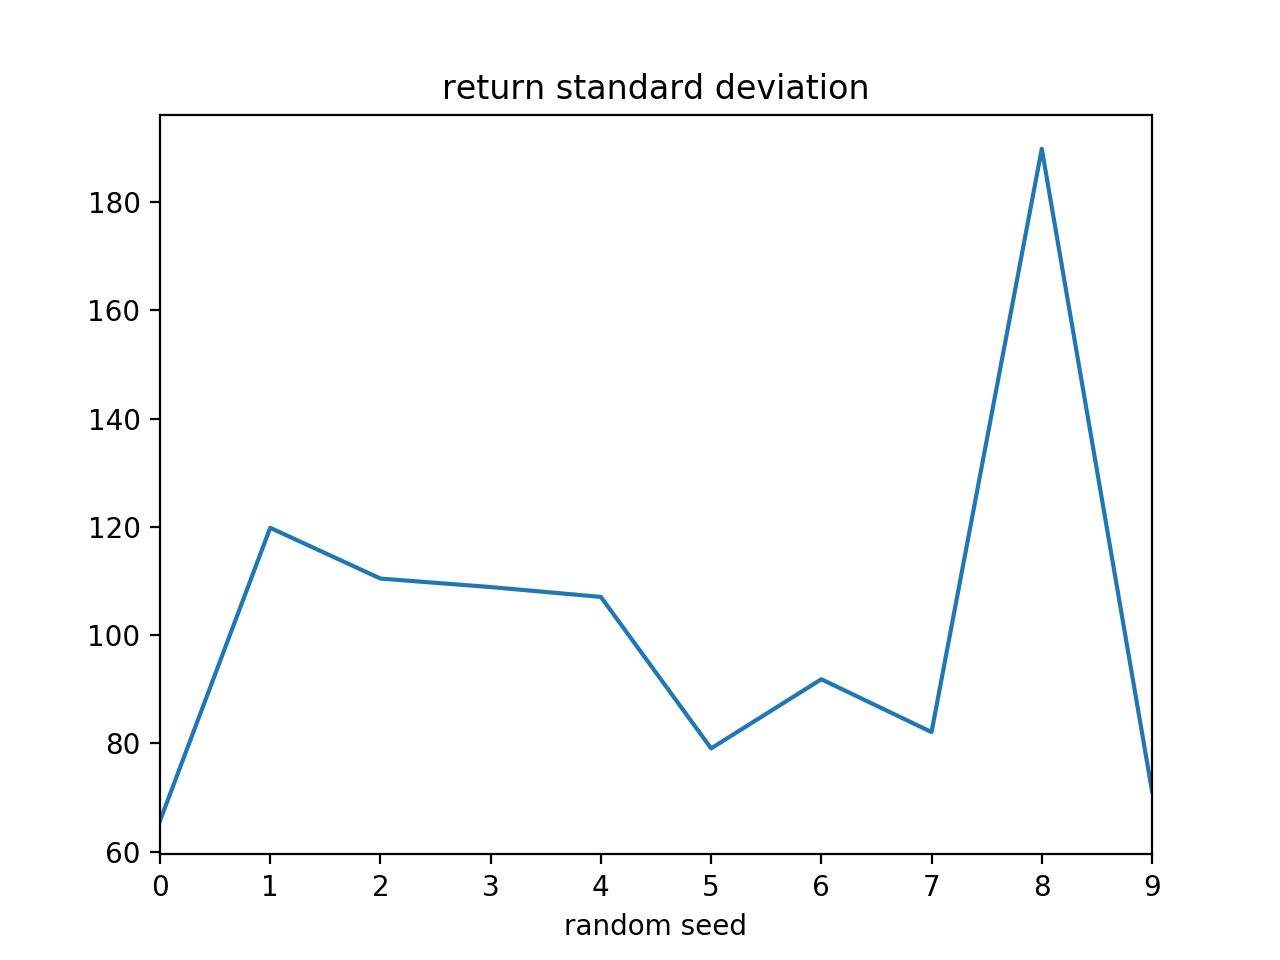
\includegraphics[width=0.95\linewidth]{return_std.png}
\captionof{figure}{}
\end{minipage}
\end{figure}

From the figure, we can clearly see a fluctuation for both the mean and the standard deviation of the returns as we vary the choice of random seed. However, the model does appear to work to some extent for all choices of random seed, suggesting that this approach is more robust than some existing DRL algorithms. A more thorough examination should require experiments for a bigger range of random seeds.

\section{DAgger}

We examine the performance of the expert policy, behavioral cloning and DAgger on the task \textbf{Walker2d-v1}. The hyperparameters are chosen as before with the random seed fixed to be $0$. We start with a collection of data from $20$ rollouts of the expert policy and add additional data from $20$ rollouts of the expert policy in each iteration of the DAgger algorithm. 

\begin{figure}[H]
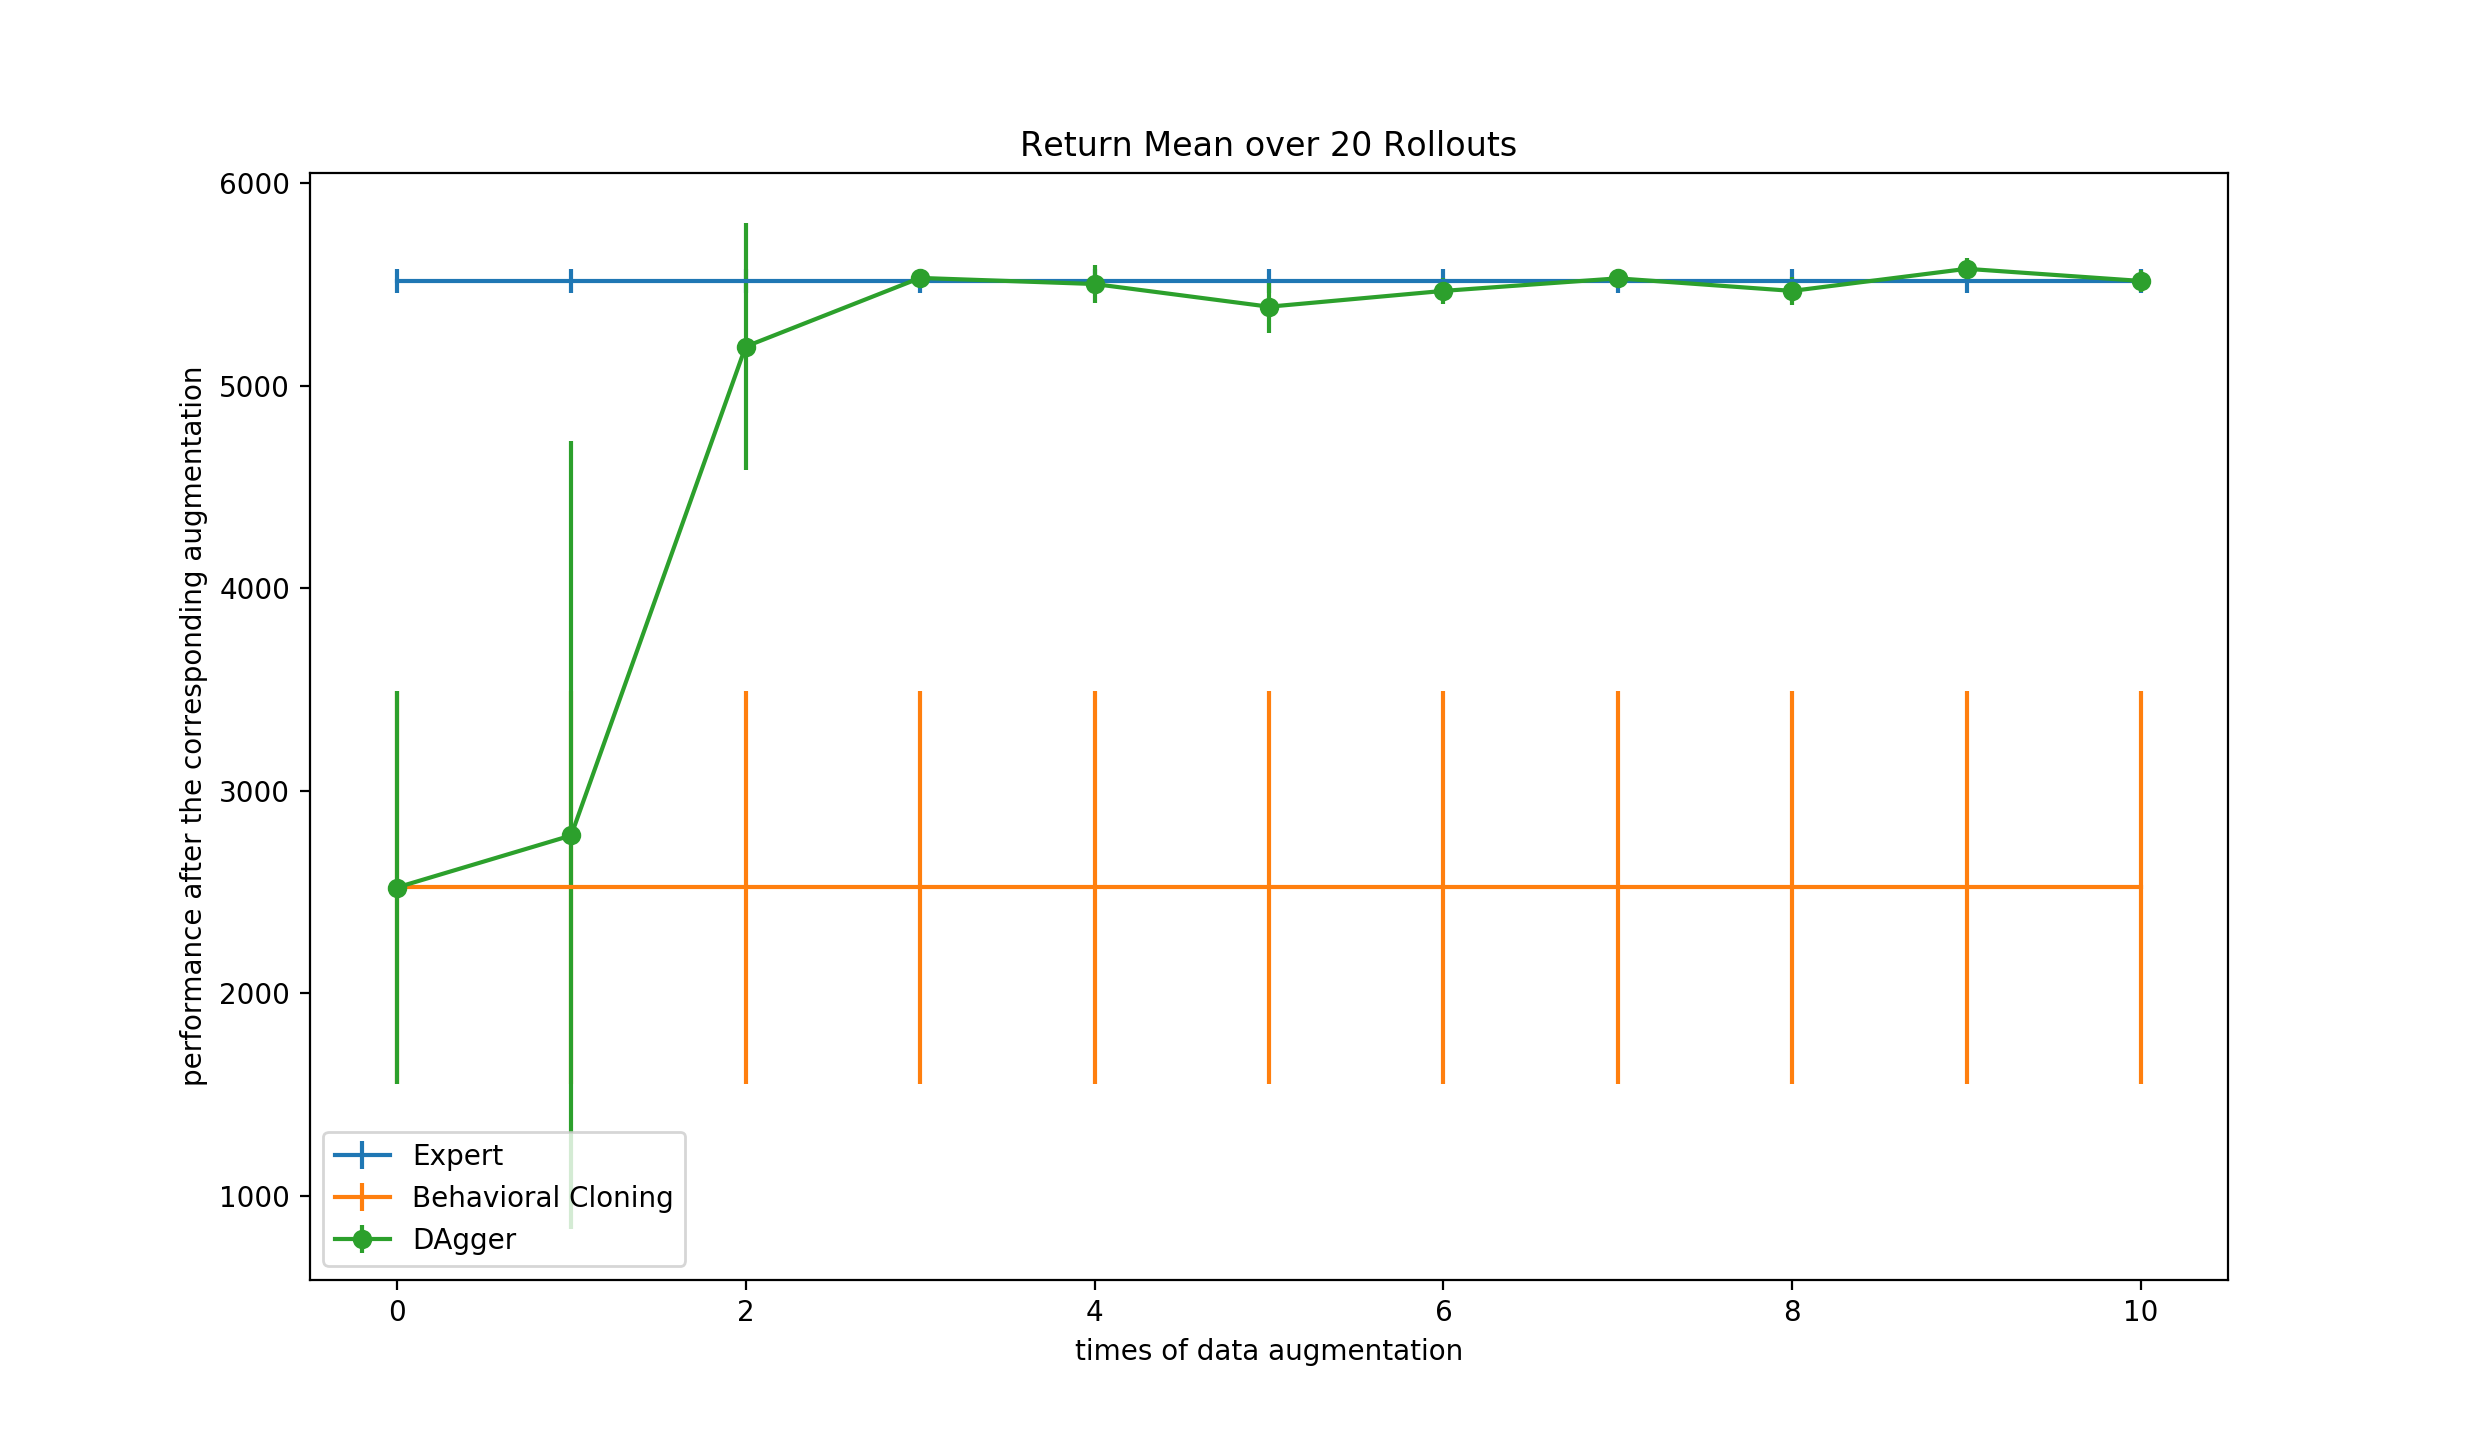
\includegraphics[width=\textwidth]{DAgger.png}
\caption{Comparison of the expert policy, naive cloned policy and policy trained using DAgger, with the vertical bars indicating the standard deviations. The performance of the expert policy and the clone policy are unrelated to the number of data augmentation performed.}
\end{figure}

\end{document}
